% !TEX encoding = UTF-8 Unicode
\documentclass{beamer}
\usetheme{Copenhagen}
\usecolortheme{dolphin}
\definecolor{lightblue}{RGB}{233, 233, 243}
\setbeamercolor{author in head/foot}{fg=black, bg=lightblue}
\setbeamercolor{title in head/foot}{bg=white}

\usepackage{url}
\usepackage{graphicx}
\usepackage{animate}
\graphicspath{{../Slike/}}
\usepackage[serbianc]{babel}
\usepackage{type1ec}
\usepackage{cmap}

\title{\textbf{\textcolor{blue}{Минимално многоугаоно раздвајање} \textcolor{red}{два скупа тачака}}}
\author{Лазар Васовић}
\institute{Математички факултет, Универзитет у Београду\\\url{https://github.com/matfija/Minimalno-razdvajanje}}
\date{25. април 2020.}

\begin{document}

\frame{\titlepage}

\begin{frame}{Поставка проблема}
\begin{itemize}
\item Два коначна скупа \textbf{\textcolor{red}{црвених}} и \textbf{\textcolor{blue}{плавих}} тачака у равни

\item Најмањи прост многоугао (тачно један) у смислу обима

\item Избор темена фиксиран на задате скупове тачака

\item Подела равни на два дела -- унутрашњост и спољашњост -- тако да су припадајуће тачке раздвојене по бојама

\item Темена су на граници -- боја им се занемарује
\end{itemize}
\end{frame}

{
\usebackgroundtemplate{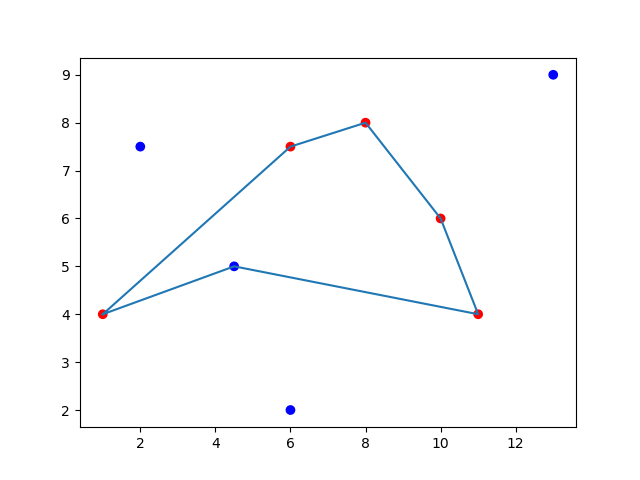
\includegraphics[width=\paperwidth]{iscrpna9.png}}
\begin{frame}
\end{frame}
}

\begin{frame}{Решавање проблема}
\begin{itemize}
\item Верзија са одлучивошћу доказано NP-тешка

\item Егзактно и (мета)хеуристичко решавање

\item Укупан број потенцијалних решења: $$\frac{1}{2} \sum_{k=3}^{n} {n \choose k} (k-1)!$$

\item Мали удео варирајуће блиских допустивих

\item Исцрпна и случајна претрага

\item Локална претрага и симулирано каљење

\item Генетски алгоритам и јато птица
\end{itemize}
\end{frame}

\begin{frame}{Претходни резултати}
\begin{itemize}
\item Рекурзивна подела простора уз динамичко програмирање

\item Произвољна темена раздвајајућег полигона:
\begin{center}
\begin{tabular}{| c | c c |} \hline
Научни рад & Сложеност & Фактор\\ \hline
$[Mata, 1995]$ & $O(n^5)$ & $O(\log k)$\\
$[Mata, 1995]$ & $O(n^2)$ & $O(\log^3n)$\\
$[Gudmundsson, 2001]$ & $O(n\log n)$ & $O(\log k)$\\
$[Mitchell, 2002]$ & $O(n^8)$ & $O(\log k)$\\
$[Mitchell, 2002]$ & $O(n^2)$ & $O(\log^2n)$\\ \hline
\end{tabular}
\end{center}

\item Фиксирана темена, али са ограничењима:
\begin{center}
\begin{tabular}{| c | c c |} \hline
Научни рад & Сложеност & Фактор\\ \hline
$[Edelsbrunner, 1988]$ & $O(n\log n)$ & $O(1)$\\
$[Edelsbrunner, 1988]$ & $O(nk)$ & $O(1)$\\
$[Eades, 1993]$ & $O(n\log n)$ & $O(1)$\\ \hline
\end{tabular}
\end{center}

\item Ознаке -- $n$ величина улаза, $k$ величина решења
\end{itemize}
\end{frame}

\begin{frame}{Нови резултати}
\begin{itemize}
\item Метахеуристике за проблем у својој пуној општости

\item Нема гаранције, па се пореде са исцрпном претрагом:
\begin{center}
\begin{tabular}{| c | c c c c c |} \hline
Тест пример & Случ. & Лок. & Каљ. & Ген. & Јато\\ \hline
\textit{ulaz9.txt} & 3 & 4 & 1 & 0 & 1\\
\textit{random1.txt} & 0 & 0 & 0 & 0 & 0\\
\textit{random2.txt} & 0 & 0 & 0 & 0 & 0\\
\textit{random3.txt} & 3 & 0 & 0 & 0 & 0\\
\textit{random4.txt} & 3 & 0 & 0 & 0 & 0\\
\textit{random5.txt} & 0 & 4 & 0 & 0 & 0\\
\textit{random6.txt} & 1 & 3 & 0 & 0 & 0\\ \hline
\end{tabular}
\end{center}

\item Мера заснована на Левенштајновом растојању

\item Фер поређење -- једнак број израчунавања погодности
\end{itemize}
\end{frame}

\begin{frame}
\animategraphics[controls,width=\linewidth]{1.2}{genetski}{01}{10}
\end{frame}

\begin{frame}{Oсновни елементи}
\begin{itemize}
\item Репрезентација -- кодирање пермутације низом тачака

\item Прилагођеност -- обим многоугла, уз евентуалну казну

\item Селекција -- случајна, турнирска, рулетска, ранговска

\item Укрштање -- првог реда, позиционо, размештање ивица

\item Мутација -- уметање, замена, обртање (инверзија), мешање, додавање, одузимање, промена тачке

\item Елитизам (20\%), случајна почетна популација, генера- цијски приступ, хибридизација са сим. каљењем
\end{itemize}
\end{frame}

\begin{frame}{Oператори јата}
\begin{itemize}
\item Оригинално прилагођавање пермутационом проблему, надахнуто радом Мориса Клерка (фр. \textit{Maurice Clerc})

\item Брзине -- низови измена, сабирање конкатенација, множење промена (углавном смањење) дужине

\item Одузимање честица -- низ измена који другу преводи у прву, заправо брзина односно растојање између њих

\item Додавање брзине честици -- примена низа трансформација на њу, уз неизбежно прескакање немогућих измена

\item Хибридизација са симулираним каљењем
\end{itemize}
\end{frame}

\begin{frame}{Имплементација}
\begin{itemize}
\item Python 3.7.6, [MSC v.1916 64 bit (AMD64)] on win32

\item Свака оптимизациона метода ручно, од нуле

\item Shapely за комфоран рад са многоугловима

\item Оригинална мера различитости између јединки
\begin{itemize}
\item Најмањи број измена које је потребно начинити да би се један многоугао свео на други, нпр. на оптимални

\item Замена -- нпр. $0 \leftrightarrow 1$ од ниске $02513$ прави $12503$

\item Дозвољено је и додавање или избацивање тачке

\item Изразита блискост -- оправдање хибридизације
\end{itemize}

\item AMD Ryzen 5 3550H 2.10 GHz, 12 GB RAM
\end{itemize}
\end{frame}

\begin{frame}{Велики пример}
\begin{itemize}
\item Досад једноцифрена кардиналност тест примера

\item Сад тридесет униформно расподељених тачака

\item Огроман простор од чак $\frac{1}{2} \sum_{k=3}^{30} {30 \choose k} (k-1)! \approx 10^{31}$ различитих многоуглова, али не много допустивих

\item Резултати упоредног извршавања алгоритама:
\begin{center}
\begin{tabular}{| c c c c c |} \hline
Случ. & Лок. & Каљ. & Ген. & Јато\\ \hline
$\infty$ & 4589 & 3733 & 3832 & 4908\\ \hline
\end{tabular}
\end{center}

\item Фер поређење -- сто хиљада евалуација погодности

\item Пронађени различити добри делови простора
\end{itemize}
\end{frame}

{
\usebackgroundtemplate{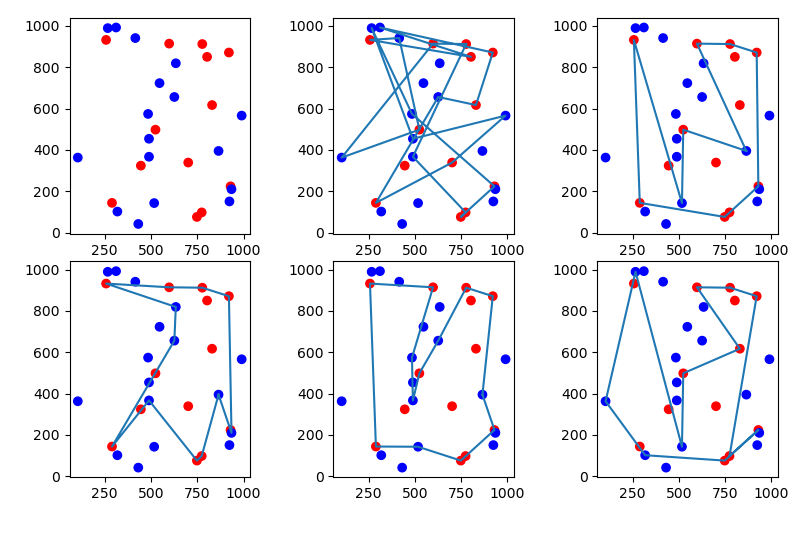
\includegraphics[width=\paperwidth,height=\paperheight]{poredjenje30v.png}}
\begin{frame}
\end{frame}
}

\begin{frame}{Закључак}
\begin{itemize}
\item Досад махом површно истражен задатак

\item Метахеуристике за проблем у својој пуној општости

\item Неколико нових идеја по питању поређења резултата

\item Најбољи генетски са симулираним каљењем

\item Класификација, рачунарски вид, избегавање судара

\item Други алгоритми, евол. стратегије, паралелизација
\end{itemize}
\end{frame}

\begin{frame}
\centering \LARGE
\textbf{ХВАЛА НА ПАЖЊИ!}

\textbf{Додатна питања?}
\end{frame}

\begin{frame}{Литература}
\nocite{*}
\bibliographystyle{amsalpha}
\bibliography{Minima\string~1}
\end{frame}

\end{document} 

